\section {Alternate DFA Representation}
\setlength{\parindent}{0pt}

(Prepared by Sameer V. Pande)

\vspace{0.3cm}


In all the modules till now, we've focussed on DFA algorithms which focus on just one variable at a time. 
For example, in constant propagation we try to propagate information about value of a variable ( $\top$/ $\bot$/ constant) throughout our CFG. 
\newline\newline
We need alternate representations of DFA because of the following reasons :
\begin{itemize}
    \item Increase the efficieny by analysing multiple variables at once.
    \item Develop a common framework/structures, with the help of which we can built a lot of DFA algorithms and reason about their properties (like optimality, precision).
\end{itemize}

Representing constant information using sets to keep track of multiple variables simultaneously is one example of alternate representation of DFA.
We store a set of tuples, where first value of tuple is the variable and the second variable is the value of the variable.
One of the optimizations of this representation is that absence of a variable from a set indicates that its value is $\bot$/. Let's see an example program to understand this alternate DFA representation.

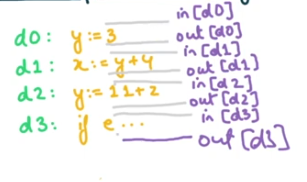
\includegraphics[scale=0.50]{88_1.png}

For each program statement, we define two program points : in and out. The information sets propagated to the program points are as follows :
\begin{itemize}
    \item \textbf{in[d0]: \{\}}
    \item \textbf{out[d0]: (in[d0] - \{(y,*)\}) $\bigcup$ \{(y,3)\}}
    \item \textbf{in[d1]: out[d0]} 
    \item \textbf{out[d1]: f(in[d1])}
    \newline where f represents the tranfer function. If f is "intelligent" then it can deduce that \textbf{x} should have value \textbf{7}. Whereas a less sophisticated would remove all tuples corresponding to variable x, since x has been overwritten
    \item \textbf{in[d2]}: out[d1]
    \item \textbf{out[d2]}: in[d2] - \{(y,*)\}
    \item and so on ...
\end{itemize}

\textbf{Meet Operator}: Meet operator is used in data-flow analysis to compute \textbf{in[node]} (\textbf{out[node]}) when there are multiple incoming (outgoing edges), with help of outsets (insets) of incoming (outgoing) edges in forward (backward) dataflow analysis.
Meet function is same as greatest-lower-bound (glb) function over the inputs. For constant-propagation the glb has to be set-intersection operator.
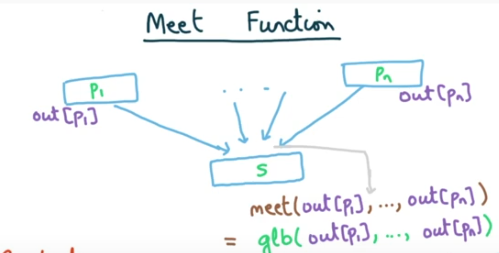
\includegraphics[scale=0.5]{88_3.png}

Summarizing the lecture, out[s] = f(in[s]), where f is the transfer-function. And very often \textbf{out[s] = (in[s] - kill[s]) $\bigcup$ gen[s]}. Note that kill and gen sets depend only on statement s. Killing before generation is also important for correctness of the analysis.